\documentclass{article}
%%%%%%%%%%%%%%%%%%%%%%%%%%%%%%%%%%%%%%%%%%%%%%%%%%%%%%%%%%%%%%%%%%%%%%%%%%%%%%%%%%%%%%%%%%%%%%%%%%%%%%%%%
\usepackage{csquotes,xpatch}% recommended
\usepackage[backend=bibtex,
style=authoryear-comp,
sortcites=false,
maxbibnames=5,maxcitenames=2,
firstinits=true,
natbib=true,
]{biblatex}

\addbibresource{refs.bib}

% natbib = true: add comma between author and year
% firstinits: for first name initials in bibliography
\renewcommand{\postnotedelim}{ } % remove comma in post citation in autocite
%\addbibresource{refs.bib}
%%%%%%%%%%%%%%%%%%%%%%%%%%%%%%%%%%%%%%%%%%%%%%%%%%%%%%%%%%%%%%%%%%%%%%%%%%%%%%%%%%%%%%%%%%%%%%%%%%%%%%%%%

% Combine label and labelyear links
\xpatchbibmacro{cite}
{\usebibmacro{cite:label}%
	\setunit{\addspace}%
	\usebibmacro{cite:labelyear+extrayear}}
{\printtext[bibhyperref]{%
		\DeclareFieldAlias{bibhyperref}{default}%
		\usebibmacro{cite:label}%
		\setunit{\addspace}%
		\usebibmacro{cite:labelyear+extrayear}}}{}{}

% Include labelname in labelyear link
\xpatchbibmacro{cite}
{\printnames{labelname}%
	\setunit{\nameyeardelim}%
	\usebibmacro{cite:labelyear+extrayear}}
{\printtext[bibhyperref]{%
		\DeclareFieldAlias{bibhyperref}{default}%
		\printnames{labelname}%
		\setunit{\nameyeardelim}%
		\usebibmacro{cite:labelyear+extrayear}}}{}{}

% Access hyperref's citation link start/end commands
\makeatletter
\protected\def\blx@imc@biblinkstart{%
	\@ifnextchar[%]
	{\blx@biblinkstart}
	{\blx@biblinkstart[\abx@field@entrykey]}}
\def\blx@biblinkstart[#1]{%
	\blx@sfsave\hyper@natlinkstart{\the\c@refsection @#1}\blx@sfrest}
\protected\def\blx@imc@biblinkend{%
	\blx@sfsave\hyper@natlinkend\blx@sfrest}
\blx@regimcs{\biblinkstart \biblinkend}
\makeatother

\newbool{cbx:link}

% Include parentheses around labelyear in \textcite only in
% single citations without pre- and postnotes
\def\iflinkparens{%
	\ifboolexpr{ test {\ifnumequal{\value{multicitetotal}}{0}} and
		test {\ifnumequal{\value{citetotal}}{1}} and
		test {\iffieldundef{prenote}} and
		test {\iffieldundef{postnote}} }}

\xpatchbibmacro{textcite}
{\printnames{labelname}}
{\iflinkparens
	{\DeclareFieldAlias{bibhyperref}{default}%
		\global\booltrue{cbx:link}\biblinkstart%
		\printnames{labelname}}
	{\printtext[bibhyperref]{\printnames{labelname}}}}{}{}

\xpatchbibmacro{textcite}
{\usebibmacro{cite:label}}
{\iflinkparens
	{\DeclareFieldAlias{bibhyperref}{default}%
		\global\booltrue{cbx:link}\biblinkstart%
		\usebibmacro{cite:label}}
	{\usebibmacro{cite:label}}}{}{}

\xpretobibmacro{textcite:postnote}
{\ifbool{cbx:link}% patch 2.7+
	{\ifbool{cbx:parens}
		{\bibcloseparen\global\boolfalse{cbx:parens}}
		{}%
		\biblinkend\global\boolfalse{cbx:link}}
	{}}
{}
{\xpatchbibmacro{textcite}% patch earlier releases
	{\setunit{%
			\ifbool{cbx:parens}
			{\bibcloseparen\global\boolfalse{cbx:parens}}
			{}%
			\multicitedelim}}
	{\ifbool{cbx:link}
		{\ifbool{cbx:parens}
			{\bibcloseparen\global\boolfalse{cbx:parens}}
			{}%
			\biblinkend\global\boolfalse{cbx:link}}
		{}%
		\setunit{%
			\ifbool{cbx:parens}
			{\bibcloseparen\global\boolfalse{cbx:parens}}
			{}%
			\multicitedelim}}
	{}{}}
%%%%%%%%%%%%%%%%%%%%%%%%%%%%%%%%%%%%%%%%%%%%%%%%%%%%%%%%%%%%%%%%%%%%%%%%%%%%%%%%%%%%%%%%%%%%%%%%%%%%%%%%%
\DeclareNameAlias{sortname}{last-first} % last name first
\renewbibmacro{in:}{} % remove in: before journal

%%%%%%%%%%%%%%%%%%%%%%%%%%%%%%%%%%%%%%%%%%%%%%%%%%%%%%%%%%%%%%%%%%%%%%%%%%%%%%%%%%%%%%%%%%%%%%%%%%%%%%%%%
\usepackage{graphicx}
\usepackage{epstopdf} 
%%%%%%%%%%%%%%%%%%%%%%%%%%%%%%%%%%%%%%%%%%%%%%%%%%%%%%%%%%%%%%%%%%%%%%%%%%%%%%%%%%%%%%%%%%%%%%%%%%%%%%%%%
\usepackage{calrsfs}
\usepackage{physics}
\usepackage{mathtools}  
\usepackage{amsmath}
\usepackage{amssymb}
\usepackage{tabulary}
\usepackage{booktabs}
\usepackage{hyperref}
%%%%%%%%%%%%%%%%%%%%%%%%%%%%%%%%%%%%%%%%%%%%%%%%%%%%%%%%%%%%%%%%%%%%%%%%%%%%%%%%%%%%%%%%%%%%%%%%%%%%%%%%%
%\usepackage{chngcntr}
%\numberwithin{equation}{chapter}
%\counterwithin{figure}{chapter}
%%%%%%%%%%%%%%%%%%%%%%%%%%%%%%%%%%%%%%%%%%%%%%%%%%%%%%%%%%%%%%%%%%%%%%%%%%%%%%%%%%%%%%%%%%%%%%%%%%%%%%%%%
\setlength{\parindent}{2em}
\setlength{\parskip}{1em}

\linespread{1.6}
\usepackage{geometry}
\geometry{
	a4paper,
	total={134mm,225mm},
	left=38mm,
	top=35mm,
	headsep=.5in
}
\raggedbottom
%%%%%%%%%%%%%%%%%%%%%%%%%%%%%%%%%%%%%%%%%%%%%%%%%%%%%%%%%%%%%%%%%%%%%%%%%%%%%%%%%%%%%%%%%%%%%%%%%%%%%%%%%
\usepackage{blindtext}
\usepackage{ragged2e}
\usepackage{float}

\usepackage{epstopdf}
\usepackage{empheq} 

\usepackage{array}
\hypersetup{
	colorlinks
}
%%%%%%%%%%%%%%%%%%%%%%%%%%%%%%%%%%%%%%%%%%%%%%%%%%%%%%%%%%%%%%%%%%%%%%%%%%%%%%%%%%%%%%%%%%%%%%%%%%%%%%%%%
\usepackage{graphics}
\graphicspath{ {figures/} }
\renewcommand{\listfigurename}{List of figures}

\usepackage[labelfont=bf,justification=justified,singlelinecheck=false]{caption}
\captionsetup[figure]{name=Fig. ,labelsep=period}
\captionsetup[table]{labelsep=period}
\captionsetup[figure]{labelfont={bf},labelformat={default},labelsep=period,name={Fig.}}
%%%%%%%%%%%%%%%%%%%%%%%%%%%%%%%%%%%%%%%%%%%%%%%%%%%%%%%%%%%%%%%%%%%%%%%%%%%%%%%%%%%%%%%%%%%%%%%%%%%%%%%%%
\usepackage{array}
\usepackage{longtable}
\usepackage{xcolor}

\usepackage{comment}

\usepackage{enumitem}

\usepackage{wrapfig}
%%%%%%%%%%%%%%%%%%%%%%%%%%%%%%%%%%%%%%%%%%%%%%%%%%%%%%%%%%%%%%%%%%%%%%%%%%%%%%%%%%%%%%%%%%%%%%%%%%%%%%%%%
\usepackage{titlesec}

\titlespacing*{\section}
{0pt}{1ex plus .5ex minus .2ex}{.5ex plus .2ex}
\titlespacing*{\subsection}
{0pt}{0.5ex plus .5ex minus .2ex}{.5ex plus .2ex}
%\titlespacing*{\subparagraph}
%{0pt}{2.5ex plus 1ex minus .2ex}{1.3ex plus .2ex}

\setcounter{secnumdepth}{4}
\setcounter{tocdepth}{4}

\newcommand{\hsp}{\hspace{5pt}}

\titleformat{\section}[block]{\bfseries\large}{\thesection}{1em}{}
\titleformat{\subsection}[block]{\bfseries\itshape}{\thesubsection}{1em}{}


%\titleformat{\subsubsection}
%{\normalfont\normalsize\itshape}{\thesubsubsection}{1em}{}
%\titleformat{\subparagraph}[runin]
%{\itshape\normalsize}{\thesubparagraph}{1em}{}

%%%%%%%%%%%%%%%%%%%%%%%%%%%%%%%%%%%%%%%%%%%%%%%%%%%%%%%%%%%%%%%%%%%%%%%%%%%%%%%%%%%%%%%%%%%%%%%%%%%%%%%%%
\usepackage{subcaption}
\usepackage{bbm}
\usepackage{tabularx}
%%%%%%%%%%%%%%%%%%%%%%%%%%%%%%%%%%%%%%%%%%%%%%%%%%%%%%%%%%%%%%%%%%%%%%%%%%%%%%%%%%%%%%%%%%%%%%%%%%%%%%%%%
\definecolor{mycolor}{RGB}{207,42,40}
\AtBeginDocument{\hypersetup{citecolor=violet, linkcolor = mycolor}}

\usepackage{indentfirst}


%%%%%%%%%%%%%%%%%%%%%%%%%%%%%%%%%%%%%%%%%%%%%%%%%%%%%%%%%%%%%%%%%%%%%%%%%%%%%%%%%%%%%%%%%%%%%%%%%%%%%%%%

\DeclareMathAlphabet{\pazocal}{OMS}{zplm}{m}{n}
\newcommand{\bw}{\boldsymbol{w}}
\newcommand{\bp}{\boldsymbol{p}}
\newcommand{\bth}{\boldsymbol{\theta}}
\newcommand{\bA}{\boldsymbol{A}}
\newcommand{\cH}{\pazocal{H}}
\newcommand{\cN}{\pazocal{N}}
\newcommand{\cP}{\pazocal{P}}
\newcommand{\cD}{\pazocal{D}}
\newcommand{\cO}{\pazocal{O}}
\newcommand{\cL}{\pazocal{L}}


\setcounter{tocdepth}{3}
\begin{document}
	
	\sloppy
	
%%%%%%%%%%%%%%%%%%%%%%%%%%%%%%%%%%%%%%%%%%%%%%%%%%%%%%%%%%%%%%%%%%%%%%%%%%%%%%%%%%%%%%%%%%%%%%%%%%%%%%%%%
	\begin{center}	
		\Large
		\textbf{Some SGD-based Bayesian ensembling approaches}\\
		\large
		Apostolos Psaros\\	
%		\today
%		July 10, 2020
	\end{center}
	\vskip 0.25in
	
%%%%%%%%%%%%%%%%%%%%%%%%%%%%%%%%%%%%%%%%%%%%%%%%%%%%%%%%%%%%%%%%%%%%%%%%%%%%%%%%%%%%%%%%%%%%%%%%%%%%%%%%%
%{\footnotesize
%\setlength{\parskip}{0.1em}
%\linespread{0.1}
%\tableofcontents
%\newpage}


%\setlength{\parskip}{1em}
%\linespread{1.6}

\section{\textcite{xie2013horizontal}: Horizontal and vertical ensemble with deep representation for classification}
One of the ensembling techniques they propose is horizontal voting; they obtain the weights at the end of each epoch and use them to make predictions. 
The weights collected can be seen as slices of the training trajectory.
An ensemble is obtained by averaging these predictions; in a sense they use this average to stabilize their prediction because of the validation set error oscillating.
They mention that this oscillation is due to the small number of training data.
The first and last epochs (i.e., the range of training epochs) they use for collecting weights are hyperparameters.
They seem to use a constant learning rate
More ensembling techniques are reviewed in \textcite{huang2017snapshot}.

\section{\textcite{smith2017cyclical}: Cyclical learning rates for training neural networks}

A minimum and maximum bound is set and the learning rate cyclically varies between them.
They note that the function according to which the rate changes does not affect significantly the performance and thus select a triangular window as shown in Fig.~\ref{triang}.
The reason for doing it is to avoid tuning the learning rate and reduce the number of training epochs; i.e., for optimization purposes.
\begin{figure}[H]
	\centering
	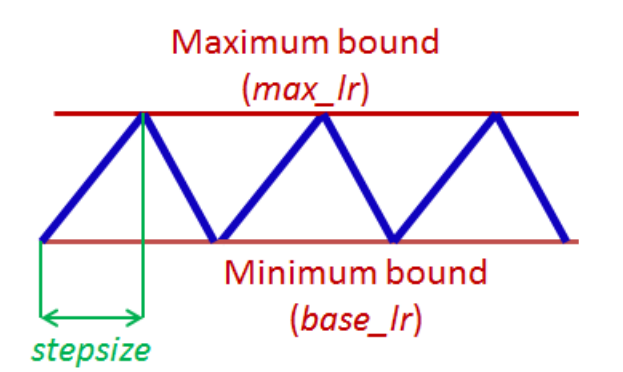
\includegraphics[width=0.5\linewidth]{./Figures/triang.png}
	\caption{Figure 2 from \textcite{smith2017cyclical}: Triangular learning rate policy. The blue lines represent learning rate values changing between bounds. The input parameter stepsize is the number of iterations in half a cycle.}
	\label{triang}
\end{figure}
After experimenting they propose to select the stepsize as $2-10$ times the number of iterations in an epoch.
For selecting the bounds the propose to run the optimization algorithm for a few epochs with linearly increasing learning rate.
By doing so the lower bound can be selected as the rate at which we see an increase to the accuracy (I guess based on the validation set) and the upper bound when it starts being ragged or decreasing. 
See Fig.~\ref{selectbounds} for an example; based on this they select the lower bound as $0.001$ and the upper bound as $0.006$.
\begin{figure}[H]
	\centering
	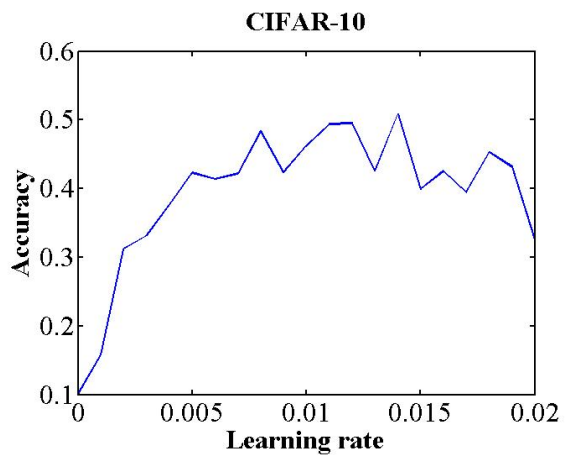
\includegraphics[width=0.5\linewidth]{./Figures/selectbounds.png}
	\caption{Figure 3 from \textcite{smith2017cyclical}: Classification accuracy as a function of increasing learning rate for 8 epochs.}
	\label{selectbounds}
\end{figure}
Finally, they note that cyclic learning rate can be combined with adaptive learning rates (e.g., AdaGrad, RMSProp, etc)

\section{\textcite{loshchilov2016sgdr}: SGDR: Stochastic gradient descent with warm restarts}
First, they review how warm restarts have been used in gradient-free and gradient-based optimization. 
In this regard, for stochastic gradient descent they simulate a warm restart by increasing the learning rate while the last weight is used as the initial solution.
They use a cosine annealing schedule that has a range of learning rates and the number of epochs until the next restart as hyperparameters.
It seems that the difference with the cyclical schedule of \textcite{smith2017cyclical} is that with cosine annealing there is also a jump in the learning rate for simulating a restart.
See also \textcite{gotmare2018using} for an empirical investigation of the type of optima obtained with SGDR and \textcite{brownlee2019snapshot} for an implementation.

The purpose of this work is primarily better convergence rate for optimization and better overall performance. 
However, during the time of this work \textcite{huang2017snapshot} published their snapshot ensembling results.
Thus, \textcite{loshchilov2016sgdr} used the weights before the last $M$ restarts and corroborated that the corresponding ``free'' ensemble leads to diverse predictions and improve performance.
They left warm restarts for AdaDelta and Adam algorithms for future work.

\section{\textcite{huang2017snapshot}: Snapshot ensembles: Train 1, get M for free}
The purpose of this paper is ensembling without incurring any additional costs as compared to standard training.
Instead of training $M$ different networks they attempt to let the SGD algorithm converge to $M$ different local optima. 
After converging to a local minumum they increase the learning rate abruptly, letting the algorithm escape the current local minimum and then decrease the rate for convergence at a different local minimum.
Before every restart they take a snapshot. 
The learning rate schedule is very similar to that of \textcite{loshchilov2016sgdr} and is changed at each iteration (not epoch). 
Note that a larger restart learning rate leads to a stronger perturbation of the weights and possibly to increased model diversity.
The budget (e.g., $300$ epochs) is divided into $M$ cycles (e.g., $M=6$) and a snapshot is collected at the end of each cycle.
See Fig.~\ref{huangschedule} for an illustration.
\begin{figure}[H]
	\centering
	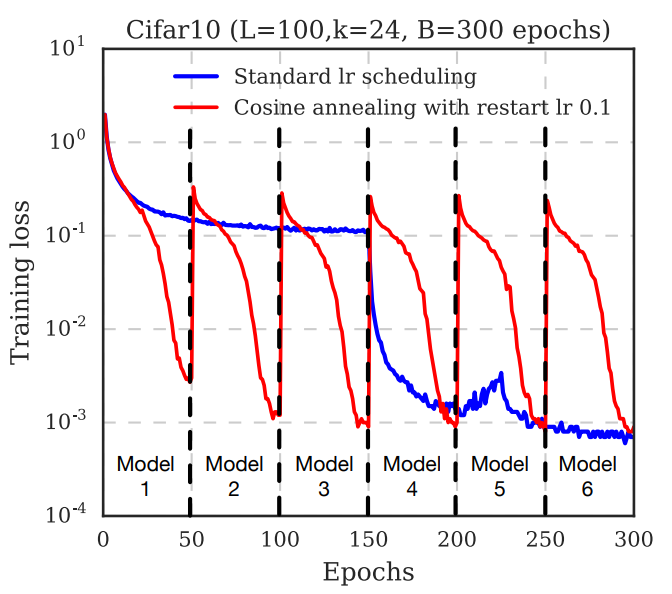
\includegraphics[width=0.5\linewidth]{./Figures/huangschedule.png}
	\caption{Figure 2 from \textcite{huang2017snapshot}: Training loss of 100-layer DenseNet on CIFAR10 using standard learning rate (blue) and M = 6
		cosine annealing cycles (red). The intermediate models, denoted by the dotted lines, form an ensemble at
		the end of training.}
	\label{huangschedule}
\end{figure}

With experiments they show the differences between snapshot ensembles (as described above), no-cycle snapshot ensembles (standard learning schedule), and single-cycle ensembles (no warm restarts, i.e., traditional ensemble with $1/M$ of the training time for each training).
In this regard, no-cycle ensembles provide less model diversity and thus, the ensemble accuracy is lower as compared to snapshot ensembles.
Further, single-cycle ensembles do not take advantage of warm restarts and thus, their ensemble accuracy is also lower as compared to snapshot ensembles.

Next, the local minima obtained are visualized for determining whether they correspond to the same basin of attraction or a different one.
Specifically, the loss along a line connecting two minima, given by $\cL(\lambda \bw_1 + (1-\lambda) \bw_2$ where $\lambda$ is a mixing coefficient, can be plotted as in Fig.~\ref{huangminima}.
As noted in the paper, two models that converge to a similar minimum (same basin of attraction) will have a smooth interpolation, whereas models that converge to different minima will likely have a spike in error for an intermediate value of $\lambda$. 
Note that this is also consistent with the results of \textcite{fort2020deep} where a line connecting two different minima is shown to pass from a region of high loss.
\begin{figure}[H]
	\centering
	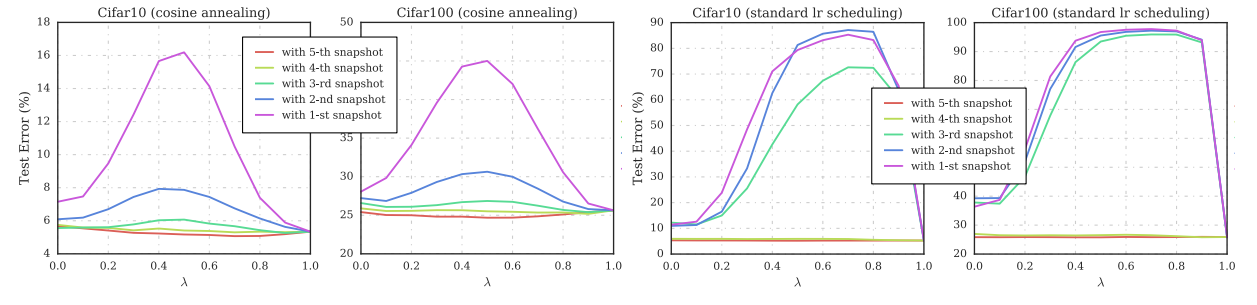
\includegraphics[width=1\linewidth]{./Figures/huangminima.png}
	\caption{Figure 5 from \textcite{huang2017snapshot}: Interpolations in parameter space between the final model (sixth snapshot) and all intermediate
		snapshots. $\lambda$ = 0 represents an intermediate snapshot model, while $\lambda$ = 1 represents the final model. Left: A
		Snapshot Ensemble, with cosine annealing cycles ($a_0$ = 0.2 every B/M = 50 epochs). Right: A NoCycle
		Snapshot Ensemble, (two learning rate drops, snapshots every 50 epochs).
}
	\label{huangminima}
\end{figure}
Overall, it appears that with cyclical learning rate most snapshots do not belong to the same basin, whereas with standard learning schedule the snapshots belong to the same basin.

Finally, model diversity is measured via pairwise correlation of outputs between any two snapshots.
A higher number corresponds to less diversity; i.e., the predictive functions do not disagree much.
As shown in Fig.~\ref{huangdiversity}, the correlation between models corresponding to adjacent snapshots is around $0.93$ and corresponding to other snapshots around $0.9$ (left).
All models also have comparable accuracy.
Therefore, they are good candidates for ensembling because we are looking for diverse and accurate predictions.
On the other hand, although snapshots obtained with standard learning rate have small correlation in the beginning they correspond to small accuracy.
And when the accuracy increases towards the fourth snapshot the correlation of the prediction is high.
Therefore, these are not good candidates for ensembling.
\begin{figure}[H]
	\centering
	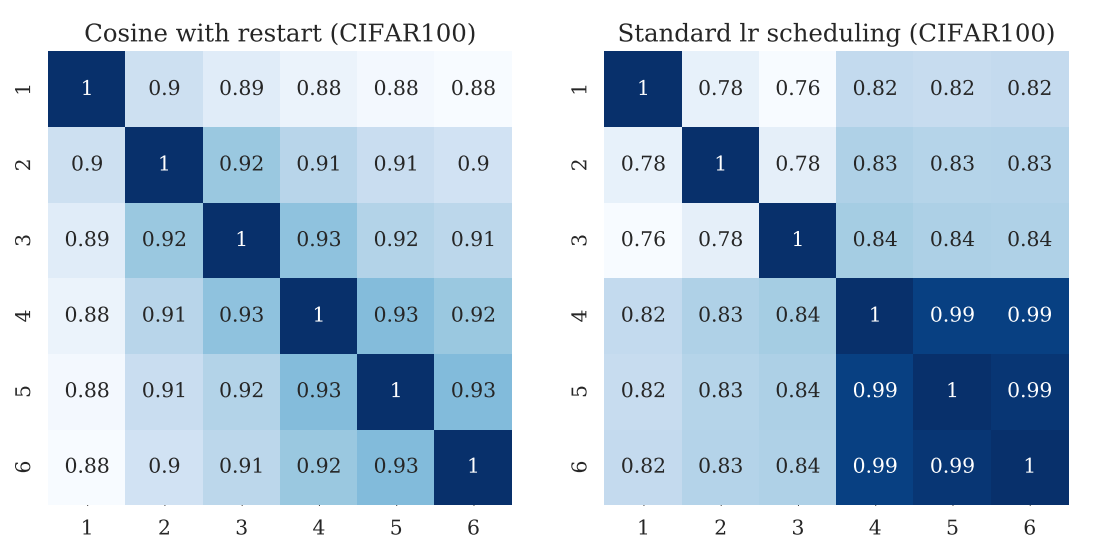
\includegraphics[width=0.7\linewidth]{./Figures/huangdiversity.png}
	\caption{Figure 6 from \textcite{huang2017snapshot}: Pairwise correlation of softmax outputs between any two snapshots for DenseNet-100. Left:A Snapshot Ensemble, with cosine annealing cycles (restart with $a_0$ = 0.2 every 50 epochs). Right: A NoCycle Snapshot Ensemble, (two learning rate drops, snapshots every 50 epochs).
}
	\label{huangdiversity}
\end{figure}

My comment: It seems that we cannot obtain uncertainty in the estimates with snapshot ensembles; it is only for increasing accuracy.
This is because we cannot obtain more than say $6-10$ samples while retaining the same computational cost as standard training.
This is the price we pay for visiting different basins of attraction. 
We need some iterations with decreasing learning rate after moving to a new basin before we are able to collect a sample.

\section{\textcite{garipov2018loss}: Loss surfaces, mode connectivity and fast ensembling of DNNs}

This paper can be divided into three parts: connecting two modes with a path, error along an obtained path and ensembling. 

\subsection{Mode connectivity}
Suppose we have two optima obtained by independently training a NN. 
We are interested in a path in the weight space connecting these two optima along which the loss is low on average. 
For doing so they consider two families of parametric curves, i.e., a polygonal chain (e.g., with two line segments and a bend in the middle) and a Bezier curve that defines a smooth path (e.g., a quadratic Bezier curve).
These curves have some parameters that define them and we can solve for the parameters that make the average loss along the path minimum. 
See Fig.~\ref{modeconnect} for an illustration. 
In the left the loss on the plane defined by three different optima is plotted, in the middle the loss on the plane\footnote{Suppose we have 3 weights $w_1, w_2, w_3$. We set $u=(w_2-w_1), v=(w_3-w_1)-\langle w_3-w_1,w_2-w_1\rangle / \norm{w_2-w_1}^2\cdot(w_2-w_1)$. Then the normalized vectors $\hat{u}=u/\norm{u}, \hat{v}=v/\norm{v}$ form an orthonormal basis in the plane containing $w_1, w_2, w_3$. To visualize the loss in this plane, we define a Cartesian grid in the basis $\hat{u}, \hat{v}$ and evaluate the networks corresponding to each of the points in the grid. 
A point $P$ with coordinates $(x,y)$ in the plane would then be given by $P=w_1+x\hat{u}+y\hat{v}$.}
defined by the two optima and (as it appears) the middle point of the Bezier curve, and in the right the loss on the plane defined by the two optima and middle point of the polygonal chain.
In all cases, connecting linearly two optima passes from a high-loss region.
Finally, although this approach relates to connecting two optima obtained by independently training the same network with the same optimizer two times, see also \textcite{gotmare2018using} for mode connectivity among pairs of networks trained with different optimizers, batch sizes, learning rate schedules etc.
\begin{figure}[H]
	\centering
	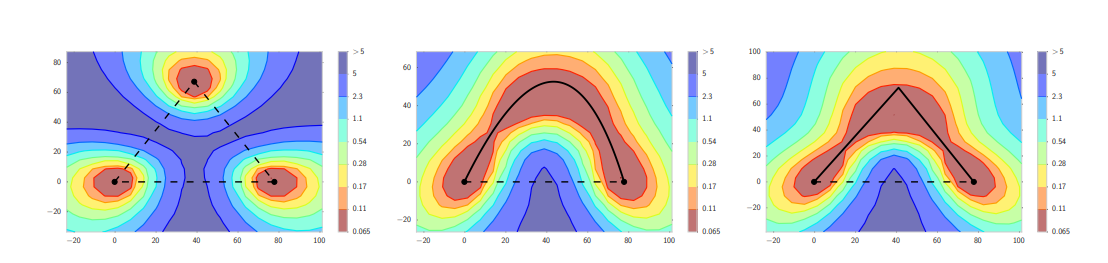
\includegraphics[width=1\linewidth]{./Figures/modeconnect.png}
	\caption{Figure 1 from \textcite{garipov2018loss}: The $l2$-regularized cross-entropy train loss surface of a ResNet-164 on CIFAR-100, as a function of network weights in a two-dimensional subspace. In each panel, the horizontal axis is fixed and is attached to the optima of two independently trained networks. The vertical axis changes between panels as we change planes (defined in the main text). Left: Three optima for independently trained networks. Middle and Right: A quadratic Bezier curve, and a polygonal chain with one bend, connecting the lower two optima on the left panel along a path of near-constant loss. Notice that in each panel a direct linear path between each mode would incur high loss.
}
	\label{modeconnect}
\end{figure}

\subsection{Loss along the obtained path}
In Fig.~\ref{huangminima} we showed that connecting with a line segment two local minima that lie in the same basin results in a training loss along the path that does not have ``barriers''.
On the other hand, a line segment connecting two local minima from different basins typically have a high-loss barrier between them.
As a result, it is interesting to plot the loss along the paths obtained as described above.
In this regard, it is shown in Fig.~\ref{lossalong} (left and middle) that the training loss and the test error remain almost constant along the obtained paths but there is a high-loss region if a line segment is used.
Most importantly, as shown in Fig.~\ref{lossalong} (right) by ensembling the network corresponding to the left end (t=0) and a network along the path (at some t) reduces the test error. 
This means that along the path the predictions are diverse, otherwise the obtained ensemble would not reduce the test error compared the single network.  
\begin{figure}[H]
	\centering
	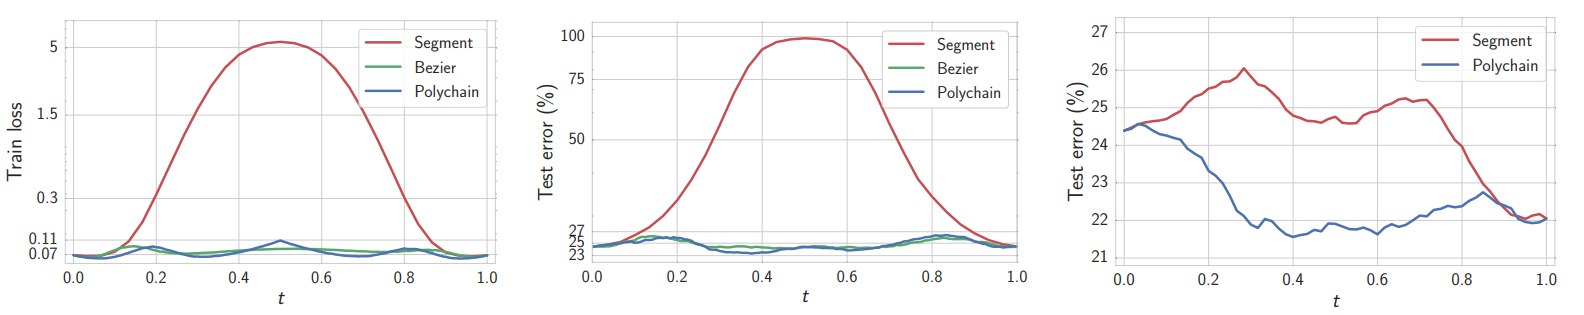
\includegraphics[width=1\linewidth]{./Figures/lossalong.png}
	\caption{Figure 2 from \textcite{garipov2018loss}: The $l2$-regularized cross-entropy train loss (left) and test error (middle) as a function of the point on the curves $\phi_{\theta}(t)$ found by the proposed method (ResNet-164 on CIFAR-100). Right: Error of the two-network ensemble consisting of the endpoint $\phi_{\theta}(0)$ of the curve and the point $\phi_{\theta}(t)$ on the curve (CIFAR-100, ResNet-164). ``Segment'' is a line segment connecting two modes found by SGD. “Polychain” is a polygonal chain connecting the same endpoints.
}
	\label{lossalong}
\end{figure}

\subsection{Ensembling}

The consequence of Fig.~\ref{lossalong} (right) is that by ensembling a model obtained by a local minimum (t=0) with a model along the polygonal chain curve (e.g., t=0.4) reduces the test error even if t is small. 
Therefore, it may be possible to reduce the test error without training a second model and without obtaining a low-loss path. 
Inspired by \textcite{smith2017cyclical} and \textcite{huang2017snapshot} the method they propose is cyclical learning rate, but with higher frequency cycles (e.g., 2-4 epochs). 
The rationale for this choice is that even by slightly perturbing the weights the obtained ensemble can reduce the test error. 
It seems that with this method the basin in which the local minimum found is explored.

On a practical note, they use a piecewise linear cyclical learning rate schedule and the local minimum is obtained with say $80\%$ of the computational budget and with a standard learning rate. 
After this pre-training phase, the rest of the computational budget is used for perturbing the weights with cyclical learning rate. 

\section{\textcite{izmailov2019averaging}: Averaging weights leads to wider optima and better generalization}
In this paper they average the weights instead of the models produced by the weights.
As a result, at test time the computational cost is not higher than a standard NN.
The weights to be averaged are obtained by SGD with constant or cyclical learning rate. 
The authors show that doing so leads to better generalization as compared to standard SGD and to comparable generalization with the ensembling method (FGE) of \textcite{garipov2018loss}.

As shown by \textcite{mandt2017stochastic}, under simplifying assumptions running SGD with constant learning rate is equivalent to sampling from a Gaussian distribution centered at the minimum of the loss. 
Whether this distribution is the posterior depends on the learning rate schedule. 
In this regard, \textcite{izmailov2019averaging} construe the SGD samples as being constrained to the surface of the sphere (because of high dimensionality) and averaging the samples allows us to go inside the sphere to find higher density solutions. 
In other words, they do not use the fact that the SGD iterates come from the posterior neither they try to sample the posterior.
Instead, they use the above as the intuition behind averaging. 
An additional intuitive explanation for averaging weights is given in Figs.~\ref{averweights} and \ref{averweights2}.
It seems that the points of the SGD trajectory are in the periphery of a set of high-performing networks. 
\begin{figure}[H]
	\centering
	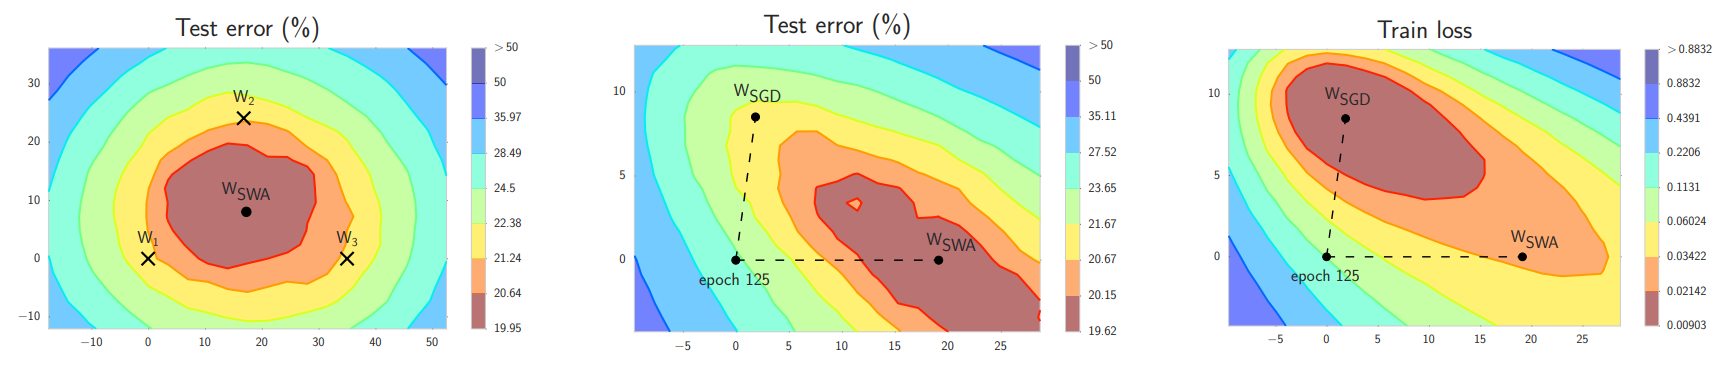
\includegraphics[width=1\linewidth]{./Figures/averweights.png}
	\caption{Figure 1 from \textcite{izmailov2019averaging}:  Illustrations of SWA and SGD with a Preactivation ResNet-164 on CIFAR-1001. Left: test error surface for three FGE samples and the corresponding SWA solution (averaging in weight space). Middle and Right: test error and train loss surfaces showing the weights proposed by SGD (at convergence) and SWA, starting from the same initialization of SGD after 125 training epochs.}
	\label{averweights}
\end{figure}
\begin{figure}[H]
	\centering
	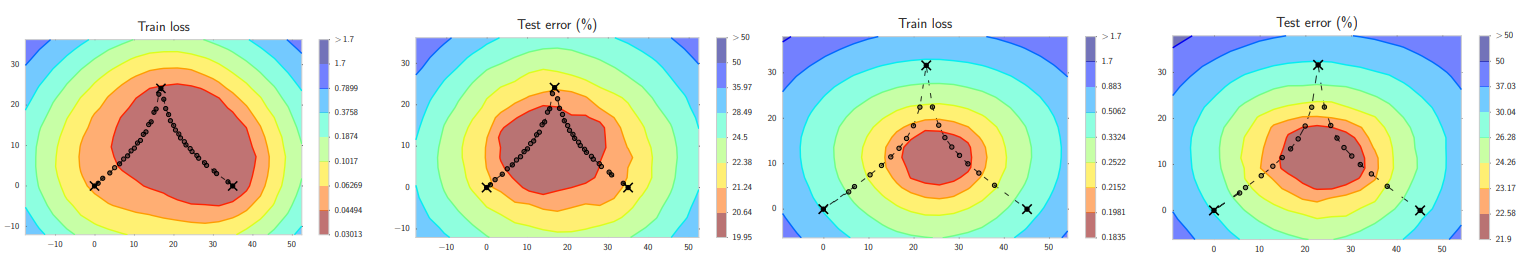
\includegraphics[width=1\linewidth]{./Figures/averweights2.png}
	\caption{Figure 3 from \textcite{izmailov2019averaging}:  The l2-regularized cross-entropy train loss and test error surfaces of a Preactivation ResNet-164 on CIFAR100 in the plane containing the first, middle and last points (indicated by black crosses) in the trajectories with (left two) cyclical and (right two) constant learning rate schedules.}
	\label{averweights2}
\end{figure}

Next, the authors show that the optimum found by averaging (SWA) corresponds to a wider solution. 
As shown in Fig.~\ref{swawider}, moving away in random directions from SWA leads to less increase in train and test loss as compared to SGD. 
\begin{figure}[H]
	\centering
	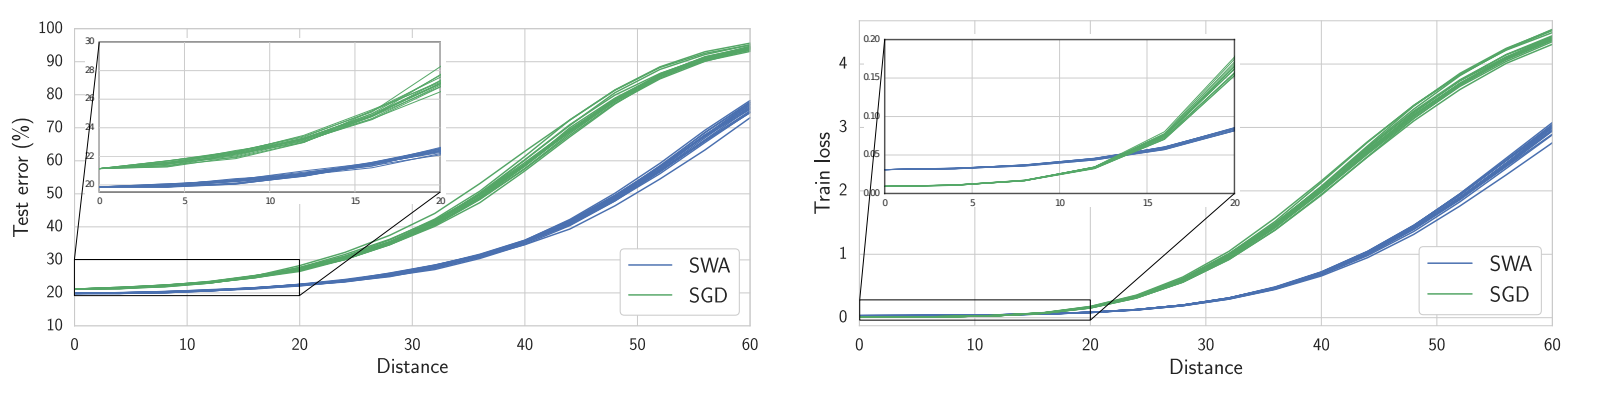
\includegraphics[width=1\linewidth]{./Figures/swawider.png}
	\caption{Figure 4 from \textcite{izmailov2019averaging}:  The l2-regularized cross-entropy train loss and test error surfaces of a Preactivation ResNet-164 on CIFAR100 in the plane containing the first, middle and last points (indicated by black crosses) in the trajectories with (left two) cyclical and (right two) constant learning rate schedules.}
	\label{swawider}
\end{figure}
This is also shown in Fig.~\ref{swawider2}. 
In the direction connecting SWA and SGD, the SGD optimum is close to a steep ascent in train and test loss. 
Although the training loss of SGD is smaller than SWA, SWA leads to better generalization. 
\begin{figure}[H]
	\centering
	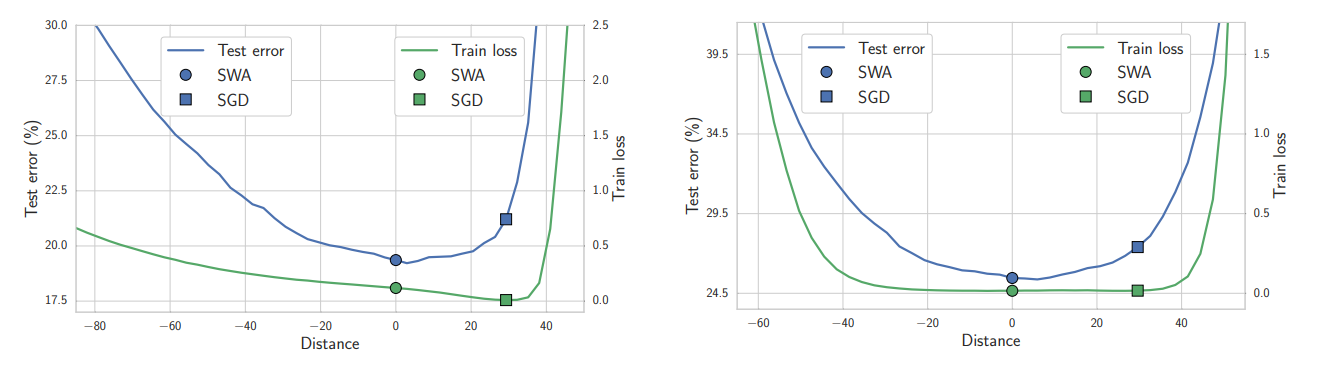
\includegraphics[width=1\linewidth]{./Figures/swawider2.png}
	\caption{Figure 5 from \textcite{izmailov2019averaging}:  l2-regularized cross-entropy train loss and test error as a function of a point on the line connecting SWA and SGD solutions on CIFAR-100. Left: Preactivation ResNet-164. Right: VGG-16.}
	\label{swawider2}
\end{figure}

My comment: What is the difference with Polyak averaging (\cite{polyak1992acceleration})?
The authors claim that Polyak averaging is not typically used for training NNs and that practitioners instead sometimes use an exponentially decaying running average of the weights found by SGD with a decaying learning rate, which smooths the trajectory of SGD but performs comparably.

\section{\textcite{maddox2019simple}: A simple baseline for Bayesian uncertainty in deep learning}

In this paper a Gaussian distribution is fitted to the iterates of SGD.
This technique is called SWAG. 
Specifically, the SWA approach of \textcite{izmailov2019averaging} is used for the mean of the distribution and two different approaches for estimating the covariance matrix are used. 
The first one is to fit a diagonal covariance matrix; a running average of the weights and of the squares of the weights is maintained (updated once per epoch) and the covariance matrix is computed at the end of training. 
The second approach is to estimate the covariance as the sum of the diagonal covariance and a low-rank matrix given as
\begin{equation}
	\Sigma = \frac{1}{M-1}\sum_{i=1}^{M}(w_i-\bar{w}_i)(w_i-\bar{w}_i)^T
\end{equation}
where $\bar{w}$ is the running average of the weights.
Note that $M$ defines the rank of the matrix and can be regarded as a hyperparameter of the method.
After fitting a covariance matrix it is easy to draw samples of the weights. 

According to \textcite{gur-ari2018gradient}, quickly during training the parameters on the trajectory are in a region where the spectrum of the Hessian separates into two components: a bulk component with many small eigenvalues and a top component of much larger positive eigenvalues. 
The large positive eigenvalues correspond to sharp directions. 
As a result, the tangent space (I guess this means where the gradient lives) has two orthogonal components, the bulk subspace and the top subspace. 
In other words, training happens in a tiny subspace and a large number of directions are left unchanged. 

For example, the SWAG technique of \textcite{maddox2019simple} fits a distribution over this low-dimensional subspace spanned by the first principal components of the SGD iterates.
Next, they claim that this fitted Gaussian distribution captures the geometry of the training loss (i.e., the posterior). 
They show that through Fig.~\ref{swaggeometry}: in the left the loss is plotted along the first principal components of the covariance matrix, in the middle the training loss is plotted around the SWA estimate and along the first two principal components and in the right along the third and the fourth. 
However, according to \textcite{gur-ari2018gradient}: ``First, the gradient of the loss during training quickly moves to lie within the top subspace of the Hessian. Within this subspace the gradient seems to have no special properties; its direction appears random with respect to the eigenvector basis''.
Therefore, is the result of Fig.~\ref{swaggeometry} just random?
In any case, the technique may still be accurate and an efficient Bayesian approximation. 
Note that the paper of \textcite{maddox2019simple} has been criticized for this reason by the reviewers of NIPS and a meta-reviewer was used who finally approved it. 
See more info at \url{http://media.nips.cc/nipsbooks/nipspapers/paper_files/nips32/reviews/7203.html}.
Finally, since there is a large number of directions that are practically not modified during training, the fitted distribution is expected to under-estimate the variances along these directions. 
However, this seems to not have significant practical implications for the approximation accuracy. 
\begin{figure}[H]
	\centering
	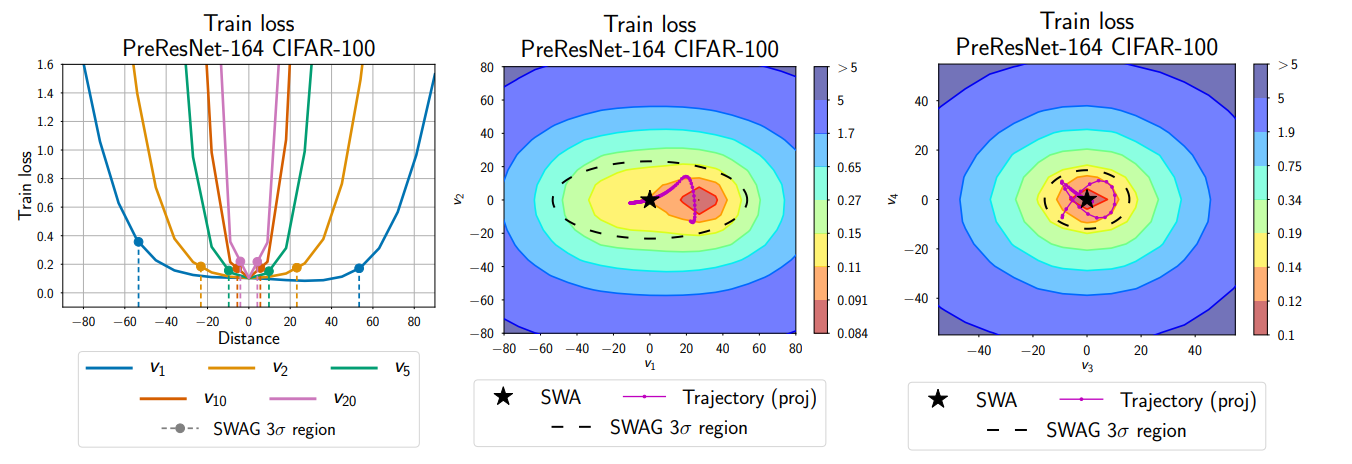
\includegraphics[width=1\linewidth]{./Figures/swaggeometry.png}
	\caption{Figure 1 from \textcite{maddox2019simple}:  Left: Posterior joint density cross-sections along the rays corresponding to different eigenvectors of SWAG covariance matrix. Middle: Posterior joint density surface in the plane spanned by eigenvectors of SWAG covariance matrix corresponding to the first and second largest eigenvalues and (Right:) the third and fourth largest eigenvalues. All plots are produced using PreResNet-164 on CIFAR-100. The SWAG distribution projected onto these directions fits the geometry of the posterior density remarkably well (see discussion).
}
	\label{swaggeometry}
\end{figure} 

\section{\textcite{izmailov2019subspace}: Subspace inference for Bayesian deep learning}
Since training happens in a tiny subspace, the authors of this paper attempt to perform approximate inference in a subspace. 
For example, \textcite{li2018measuring} attempts to perform training in a randomly oriented small subspace and define a size above which the accuracy difference is not significant.
Thus, the first thing \textcite{izmailov2019subspace} try is to perform inference in a random subspace centered at the SWA estimate (this is an affine space).
So they select a small number of random dimensions, create an affine space centered at the SWA estimate and perform inference in this subspace; i.e., obtain a distribution over this low-dimensional subspace. 
So the obtained weight samples after inference will belong to this subspace only and follow the distribution obtained via inference.

Another approach is to perform inference on the subspace defined by the first PCA components of the SGD iterates. 
This is similar to the technique of \textcite{maddox2019simple} but instead of fitting a Gaussian distribution they perform inference in the subspace. 
Further, they perform inference in the curve subspace discussed in \textcite{garipov2018loss}.
Note, however, that not only one has to construct this curve subspace (by finding a connecting path) but then also perform inference. 

Finally, note that because the subspaces discussed above are very low-dimensional and there are much more training datapoints the posterior of this inference concentrates and thus leads to overconfident uncertainty estimates. 
For this reason, they use a tempered posterior, i.e., raise the likelihood to a power.
This power is a hyperparameter to be determined through cross-validation.







 

%%%%%%%%%%%%%%%%%%%%%%%%%%%%%%%%%%%%%%%%%%%%%%%%%%%%%%%%%%%%%%%%%%%%%%%%%%%%%%%%%%%%%%%%%%%%%%%%%%%%%%%%%	

%\section*{Appendix}
\newpage	
\printbibliography[heading=bibintoc,title={References}]
	
\end{document}